% Remember to insert \end{doublespacing} somewhere after this... not necessarily in the same .text file though
% \begin{doublespacing}

% \part{ Appendix}\label{part:appendices}
\chapter{Mechanical drawings}\label{ch:mech_drawings}

This appendix contains reproductions of mechanical drawings for some key components of the apparatus(es) described in this thesis.

\newpage

\begin{sidewaysfigure}[!t]
    \centering
    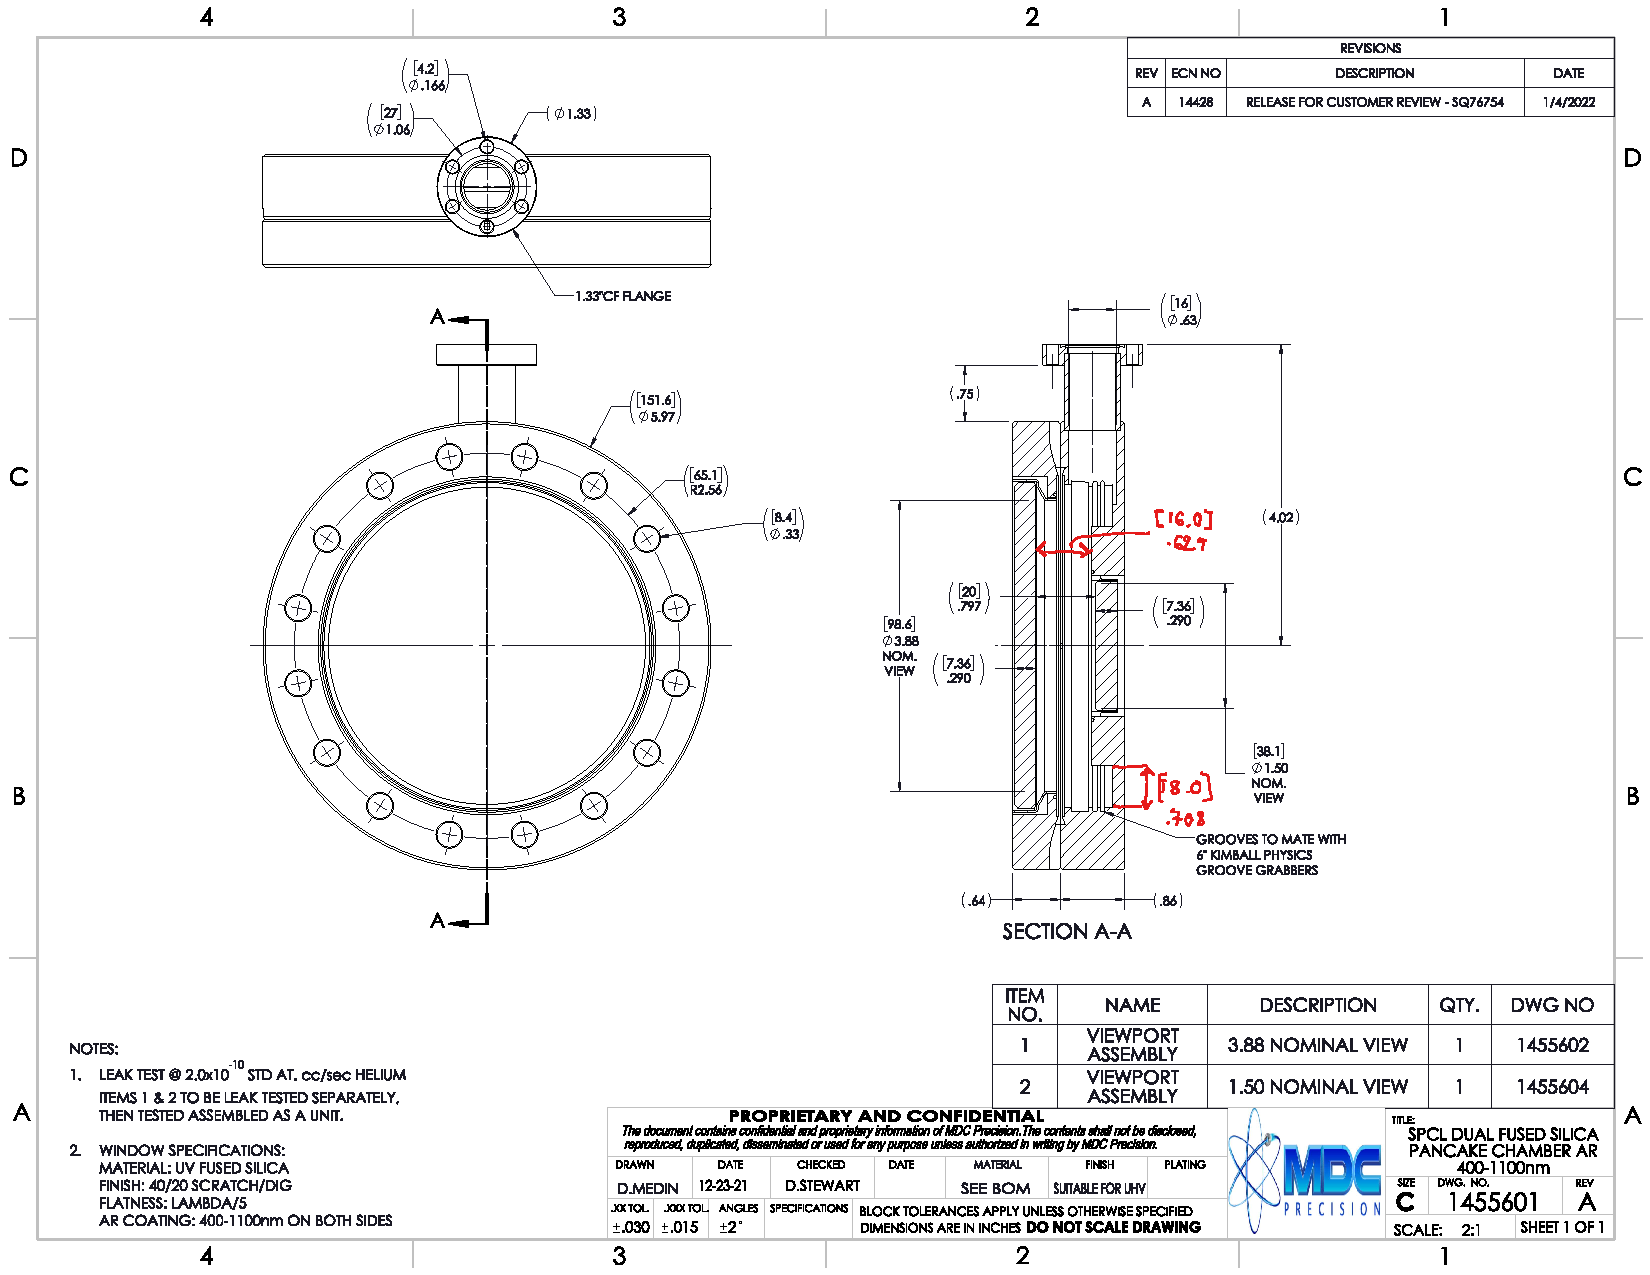
\includegraphics[width=1\textwidth]{Images/mdc_chamber_20220428.pdf}
    \caption{Mechanical drawing of the ultra-high vacuum science chamber from MDC Precision. The annotations in red were added to the original drawing provided by MDC to determine previously unspecified dimensions}.
    \label{fig:drawing_mdc_chamber}
\end{sidewaysfigure}

\newpage

\begin{sidewaysfigure}[!ht]
    \centering
    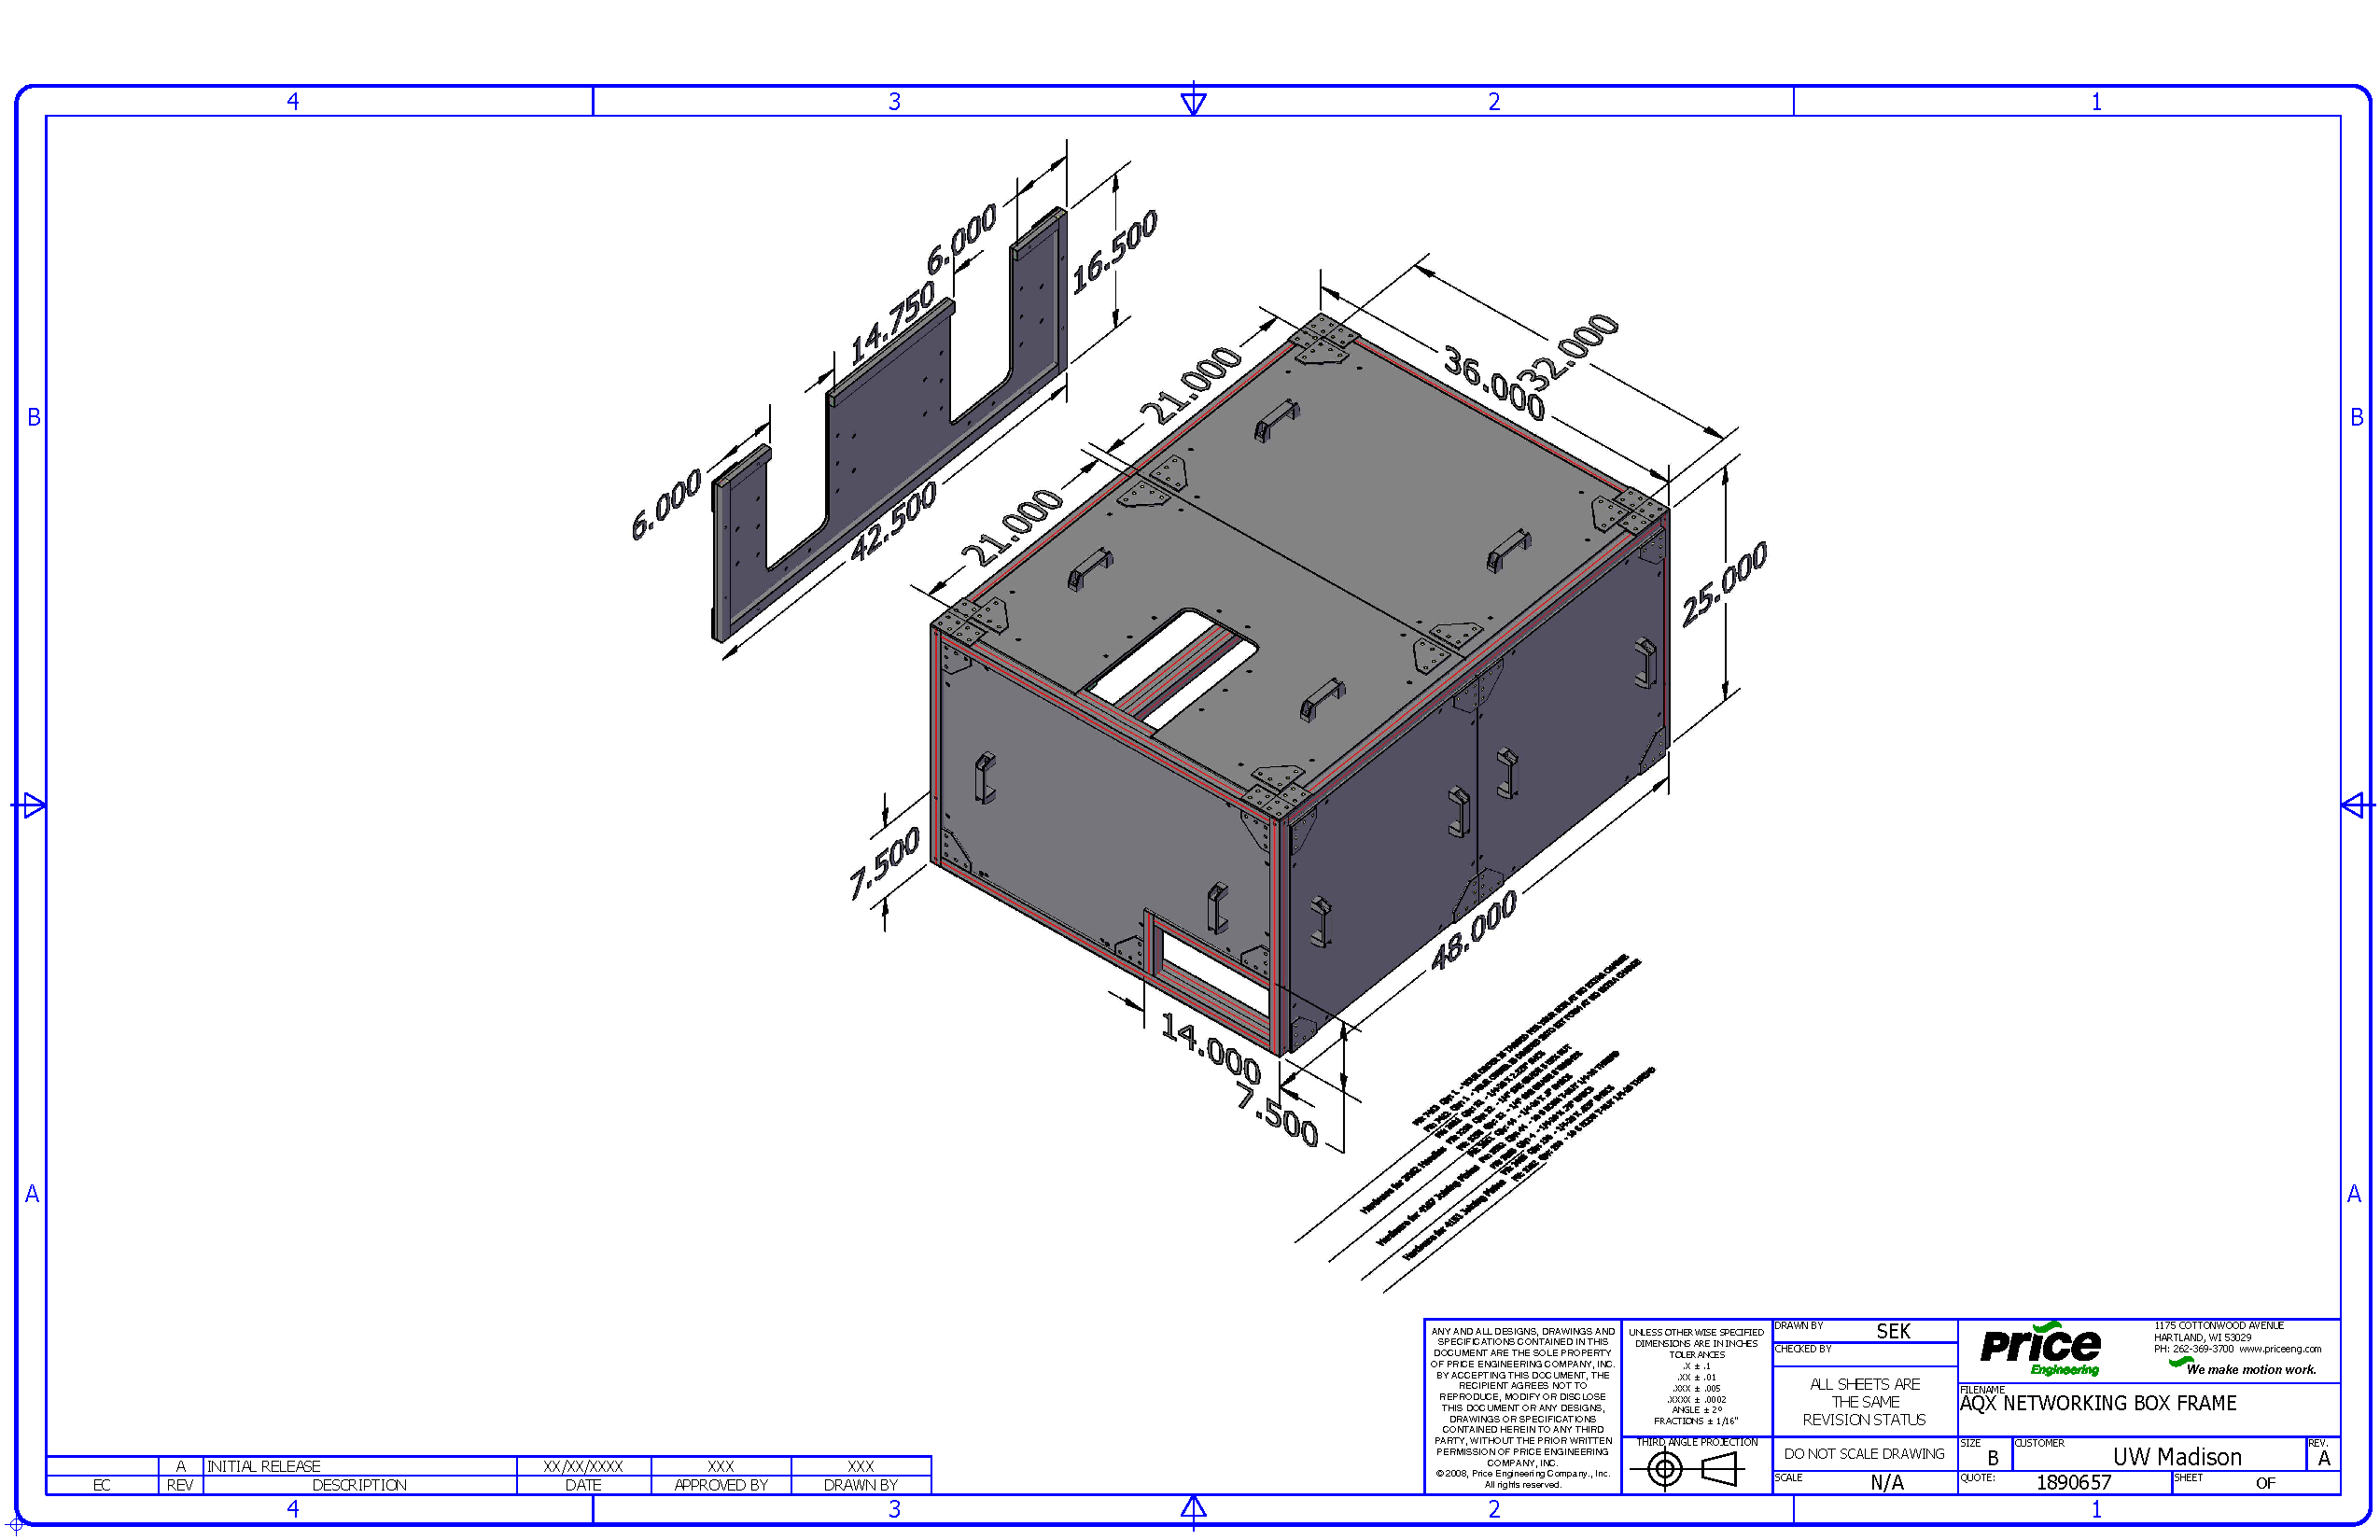
\includegraphics[width=1\textwidth]{Images/AQX Networking Box Frame LAYOUT.pdf}
    \caption{CAD drawing of the experiment box courtesy of Price Engineering. The slots in the top and back panels are for attaching cable feedthrough panels.}
    \label{fig:experiment_box_frame}
\end{sidewaysfigure}

% \begin{sidewaysfigure}[!t]
%     \centering
%     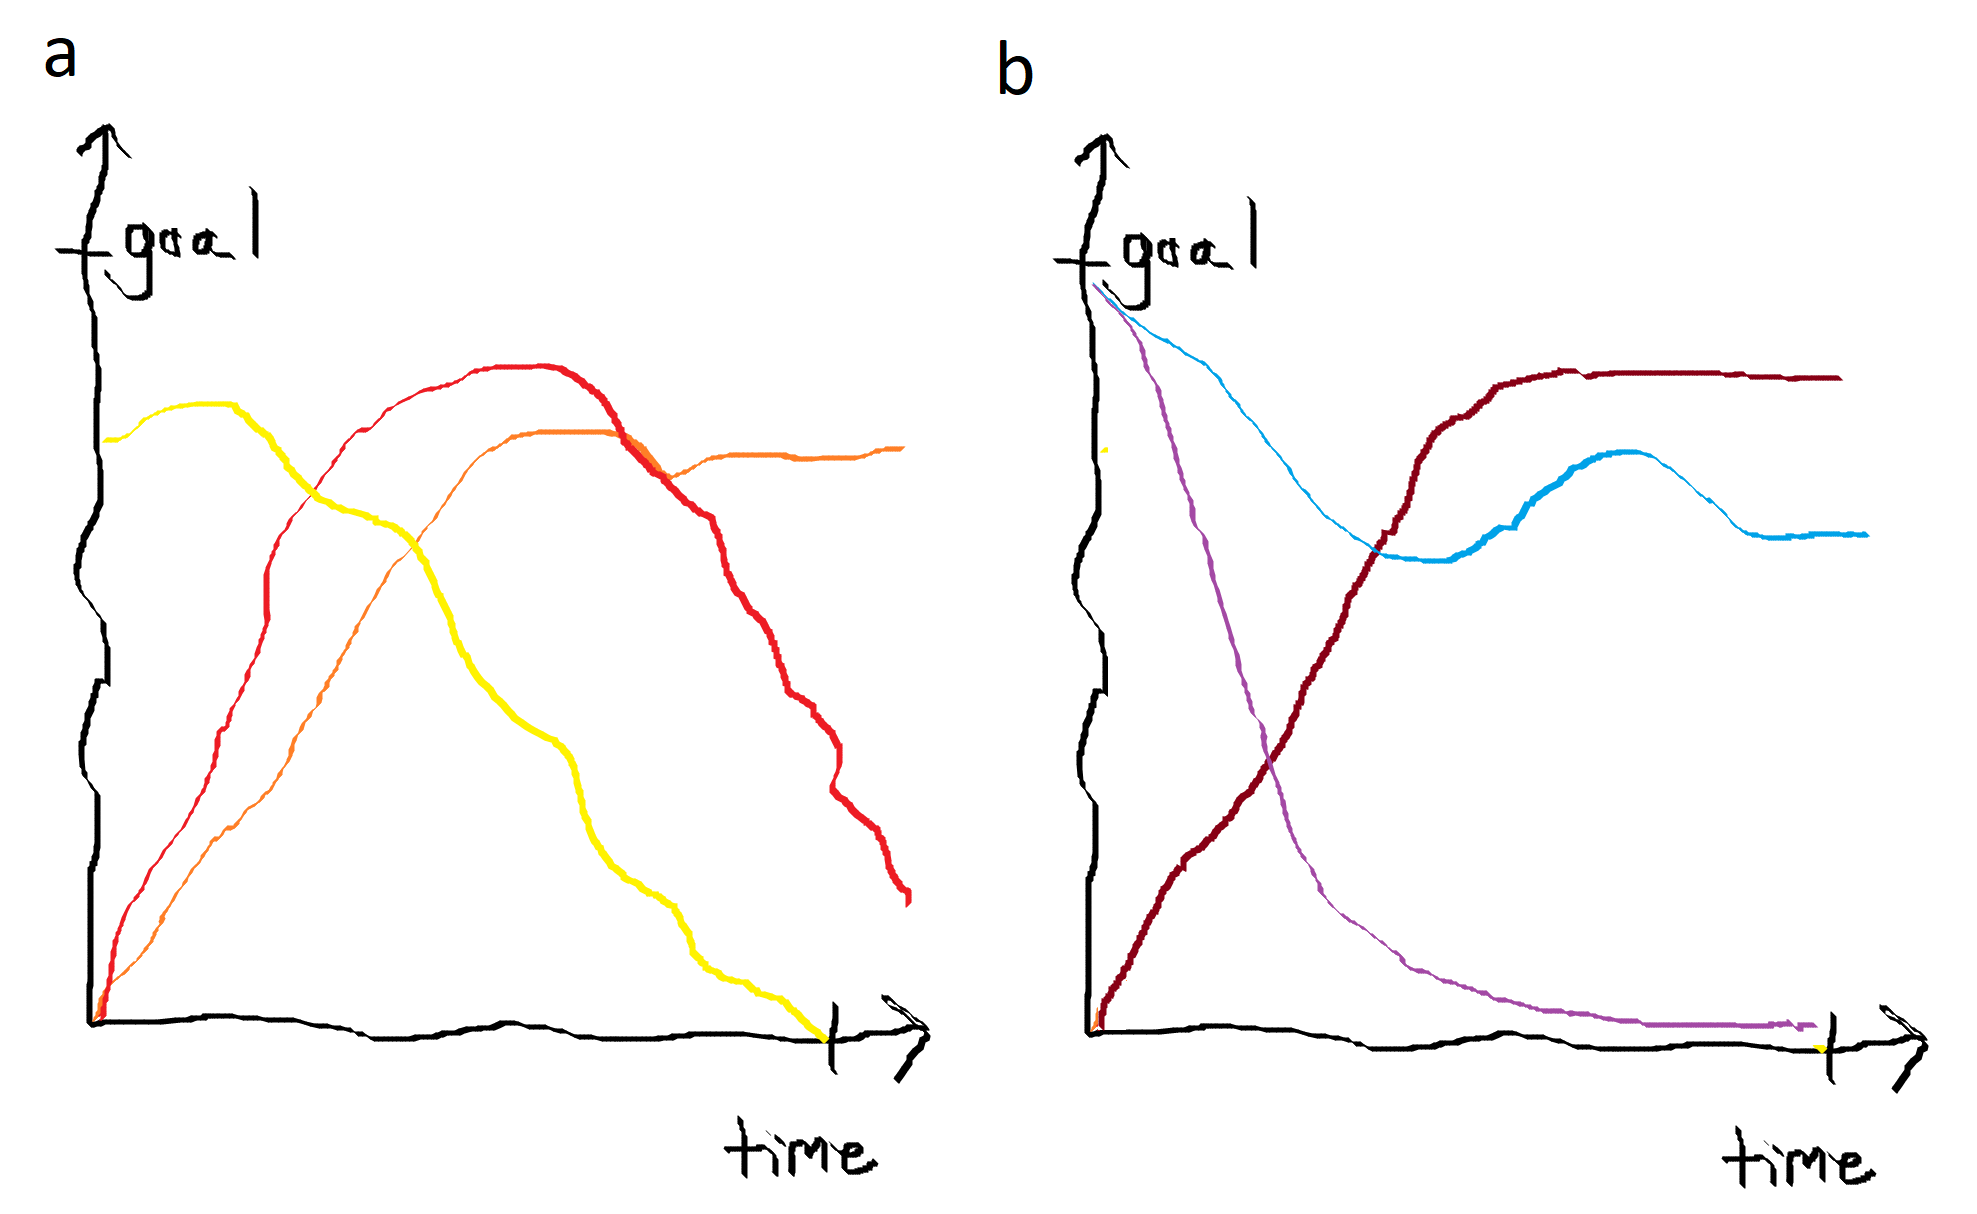
\includegraphics[width=1\textwidth]{Images/fig_coming_soon.png}
%     \caption{Mechanical drawing of the MACOR substrate or ``bridge" for the parabolic mirror version of the experiment design}.
%     \label{fig:macor_bridge_mirror}
% \end{sidewaysfigure}

\newpage

\begin{sidewaysfigure}[!t]
    \centering
    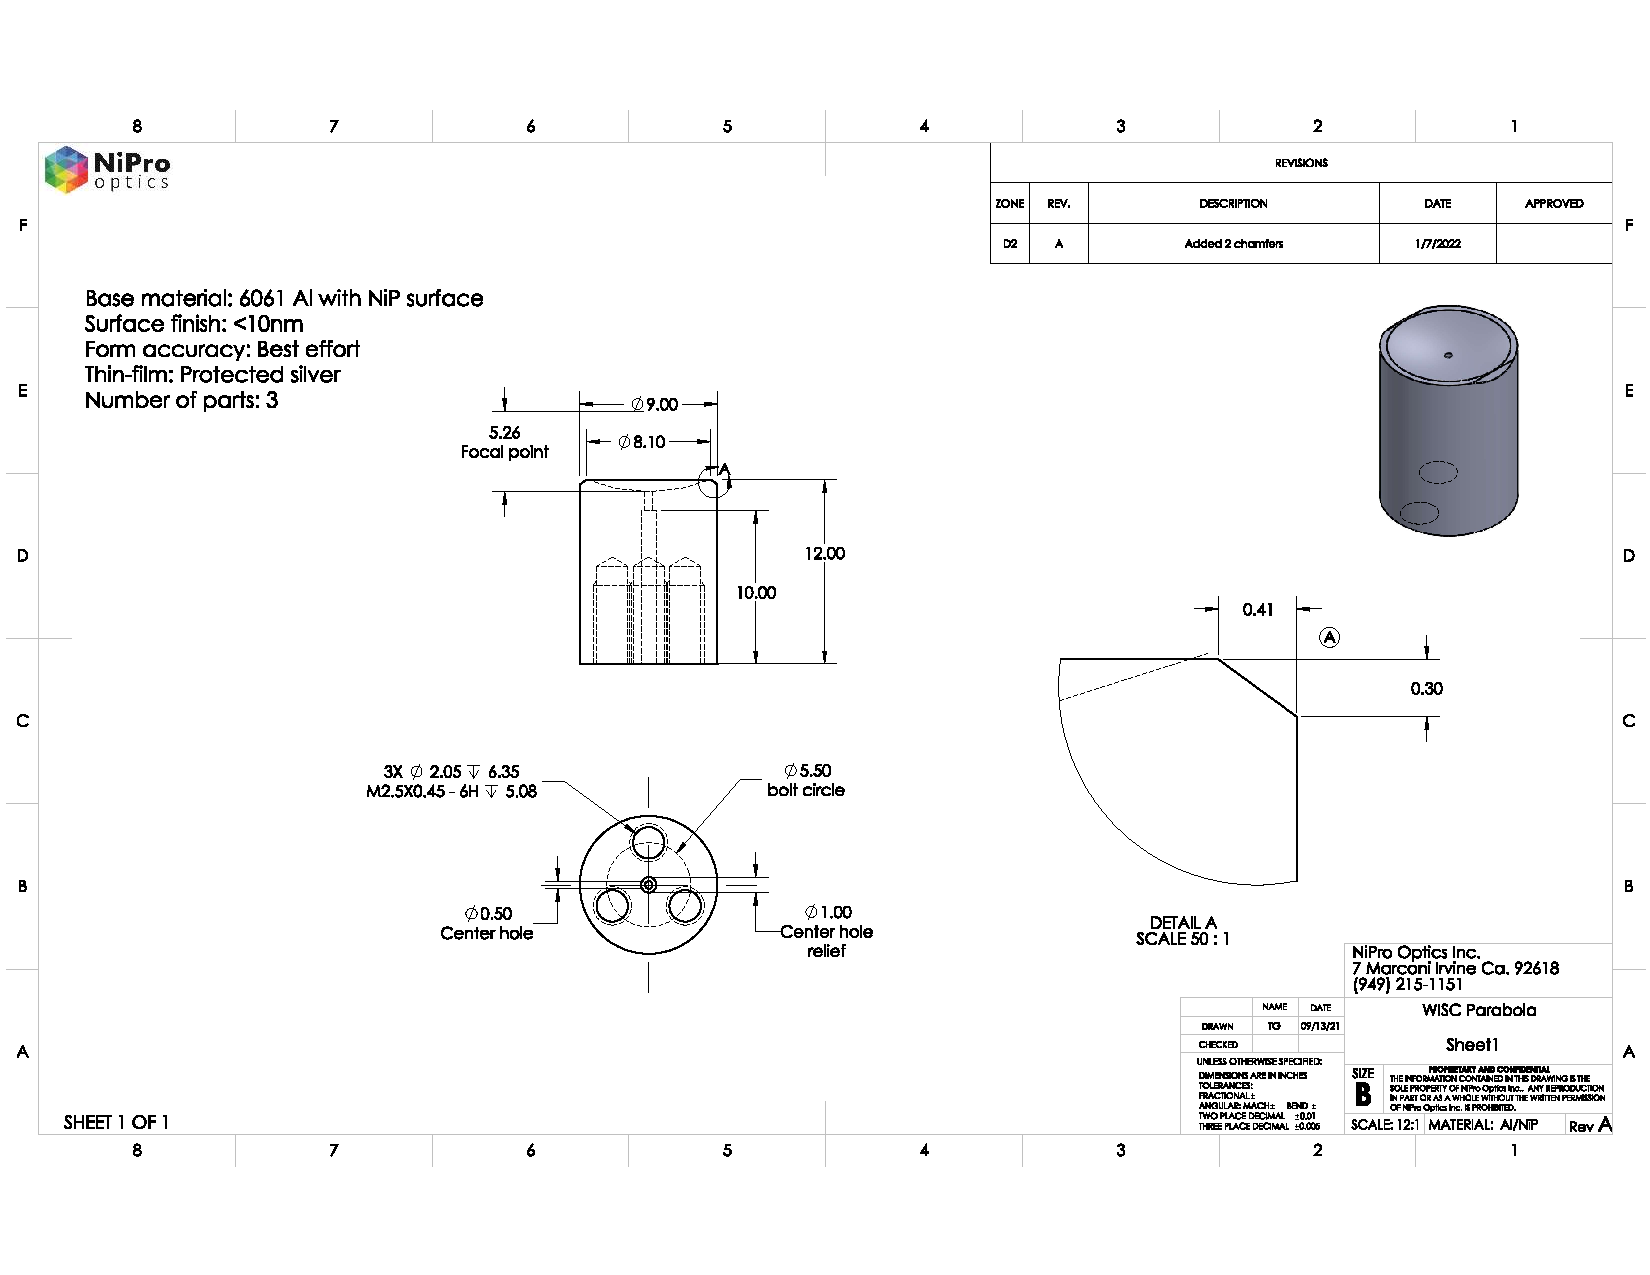
\includegraphics[width=1\textwidth]{Images/nipro_parabolic_mirror_drawing.pdf}
    \caption{Mechanical drawing of the parabolic mirror used as the focusing optic for both the dipole trap and photon collection in a quantum network node. The mirror was coated with a layer of nickel and then protected silver}.
    \label{fig:mirror}
\end{sidewaysfigure}
